\documentclass{beamer}
\usetheme{Singapore}
\setbeamercovered{transparent}

\usepackage{ dsfont }
\usepackage{ amsmath }
\usepackage{ mathrsfs }
\usepackage{ amssymb }
\usepackage{ amsthm }
\usepackage{ graphicx }
\usepackage{tikz}
\usepackage[font=scriptsize,labelfont=bf]{caption}
\usepackage{xcolor}

\usepackage[utf8]{inputenc}

\newcommand{\Prob}{\mathbb{P}}
\DeclareCaptionFont{tiny}{\tiny}
\DeclareCaptionFont{blue}{\color{blue}}
\setbeamertemplate{caption}[numbered]
\newcommand{\PP}{\mathbb{P}}
\newcommand{\R}{\mathbb{R}}
\newcommand{\cd}{\overset{d}{\longrightarrow}}
\newcommand{\Floor}[1]{{\lfloor {#1} \rfloor}}


\AtBeginSection[]
{
	\begin{frame}
		\frametitle{Table of Contents}
		\tableofcontents[currentsection]
	\end{frame}
} 
 
 
%Information to be included in the title page:
\title{Inference on Heavy-Tailed\\ Max-Renewal Processes}
%\subtitle{}
\author{Smarak Nayak}
\date{October 28, 2016}
 
 
\begin{document}
 
\frame{\titlepage}
\section{Introduction}

\begin{frame}{Motivation}
	Classical extreme value theory assumes that events happen uniformly. \\~\\
	
	However this is not always the case, in many systems the events occur in bursts. \\~\\
	
	Examples include both human-created events and physical phenomena:
		\begin{itemize}
		\item Communication
		\item Financial Trades 
		\item Network Traffic
		\item Neuron Firing Sequences
		\item Seismic Activity
	    \end{itemize}
	
\end{frame}

\begin{frame}{Example Processes}
	
    \begin{figure}
    	\captionsetup{font=tiny,width=0.9\textwidth,labelfont={blue,bf}}
        \centering
        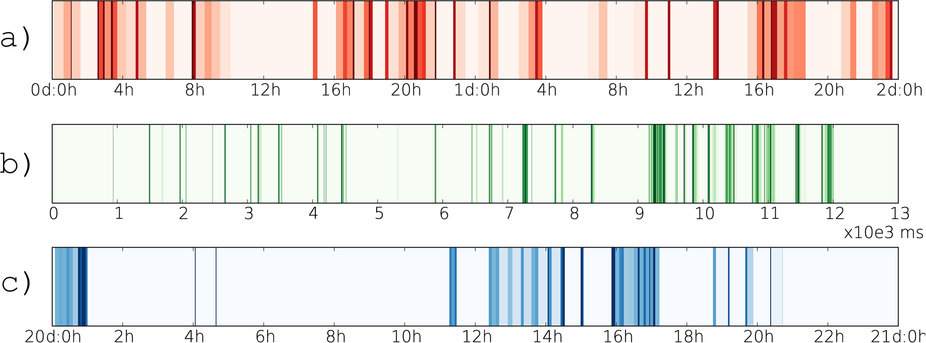
\includegraphics[scale=1.4]{BurstyGraphs}
        \caption{(a): Sequence of earthquakes with magnitude larger than two at a single location (South of Chishima Island, 8th–9th October 1994) (b): Firing sequence of a single neuron (from rat's hippocampal) (c): Outgoing mobile phone call sequence of an individual. The darker the colour the shorter the time between consecutive events. (Karsai, Kaski, Barabási \& Kertész, 2012)}
    \end{figure}
\end{frame}
 
\begin{frame}{Notation}
	
	Let $J_1 , J_2 , ...$ be a sequence of i.i.d. random variables that model the jump sizes (event magnitudes).
	\\~\\
	Let $W_1, W_2, ...$ be a sequence of i.i.d positive random variables that model the waiting times between the jumps.
	\\~\\
	We can then define $(W_1 , J_1 ), (W_2 , J_2 ), ...$ to be a sequence of i.i.d $\mathbb{R} \times \mathbb{R} ^+$ random variables.
\end{frame}

\begin{frame}{Notation Contd.}
    Now define $S(n):=\sum^n_{i=1} W_i$ as the partial sum of the first $n$ waiting times.
    \\~\\
    Define a renewal process $N(t):=\max\{n\geq0:S(n)\leq t\}$.
    \\~\\
    Define $M(n):=\bigvee_{k=1}^{n} J_k$ as the partial maxima of the first $n$ jumps.
    \\~\\
    Finally we define the Continuous Time Random Maxima (CTRM) to be $M(N(t)) := \bigvee_{k=1}^{N(t)} J_k
= \max\{J_k: k = 1, \ldots, N(t)\}.$
\end{frame}

\begin{frame}{CTRM Example}
\begin{figure}
\centering
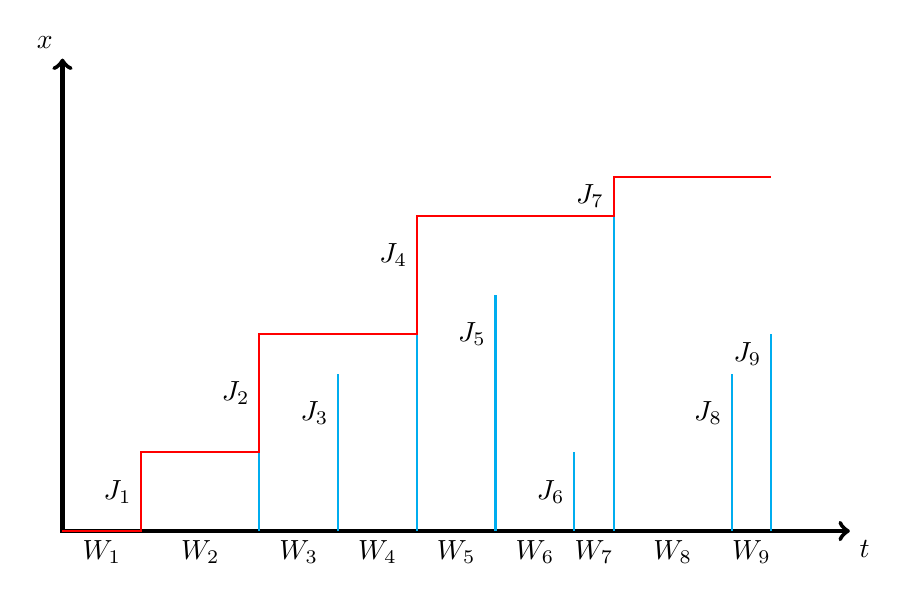
\begin{tikzpicture}
	\draw[ultra thick][<->] (0,6)--(0,0)--(10,0);
	\draw[thick][cyan] (1,0)--(1,1);
	\draw[thick][cyan] (2.5,0)--(2.5,2.5);
	\draw[thick][cyan] (3.5,0)--(3.5,2);
	\draw[thick][cyan] (4.5,0)--(4.5,4);
	\draw[thick][cyan] (5.5,0)--(5.5,3);
	\draw[thick][cyan] (6.5,0)--(6.5,1);
	\draw[thick][cyan] (7,0)--(7,4.5);
	\draw[thick][cyan] (8.5,0)--(8.5,2);
	\draw[thick][cyan] (9,0)--(9,2.5);
	\node [above left] at (0,6) {$x$};
	\node [below right] at (10,0) {$t$};
	\node [left] at (1,0.5) {$J_1$};
	\node [below] at (0.5,0) {$W_1$};
	\node [left] at (2.5,1.75) {$J_2$};
	\node [below] at (1.75,0) {$W_2$};
	\node [left] at (3.5,1.5) {$J_3$};
	\node [below] at (3,0) {$W_3$};
	\node [left] at (4.5,3.5) {$J_4$};
	\node [below] at (4,0) {$W_4$};
	\node [left] at (5.5,2.5) {$J_5$};
	\node [below] at (5,0) {$W_5$};
	\node [left] at (6.5,0.5) {$J_6$};
	\node [below] at (6,0) {$W_6$};
	\node [left] at (7,4.25) {$J_7$};
	\node [below] at (6.75,0) {$W_7$};
	\node [left] at (8.5,1.5) {$J_8$};
	\node [below] at (7.75,0) {$W_8$};
	\node [left] at (9,2.25) {$J_9$};
	\node [below] at (8.75,0) {$W_9$};
	\only<2>{
	\draw[thick][red](0,0)--(1,0)--(1,1)--(2.5,1)--(2.5,2.5)--(4.5,2.5)--(4.5,4)--(7,4)--(7,4.5)--(9,4.5);
	}
\end{tikzpicture}
\end{figure}
\end{frame}

\section{Scaling Limits}

\begin{frame}{Discrete Random Walk}
	\begin{figure}
		\captionsetup{font=tiny,width=0.9\textwidth,labelfont={blue,bf}}
		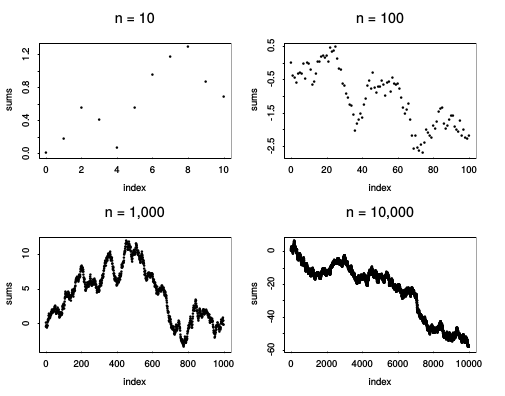
\includegraphics[scale=0.65]{Thesis/Figures/RandomWalk}
		\caption{Possible realisations of a random walk with steps, $U_i$, uniformly distributed in $[1/2,1/2]$}
	\end{figure}
\end{frame}

\begin{frame}{A Continuous Analogue}
	We seek a continuous  function that coincides with the Discrete Random Walk at integer arguments.
\\~\\
There are two obvious choices:
		\begin{itemize}
		\item A linear interpolation between every point
		\item The step function $S_{\lfloor t \rfloor}=U_1+\cdots+U_{\lfloor t \rfloor}$\newline
	    \end{itemize}
Both are equivalent for large $t$ so we consider the step function as it's simpler.
\\~\\
Now add a time scaling constant $c$ such that $S_{\lfloor ct \rfloor}=U_1+\cdots+U_{\lfloor ct \rfloor}$.
\end{frame}

\begin{frame}{The Classical Functional Central Limit Theorem}
Recall that the classical Central Limit Theorem states
\[
\frac{S_n-n\mu}{\sqrt{n\sigma^2}}\overset{d}{\longrightarrow}Z\sim N(0,1)\textrm{ as $n\to\infty$}.
\]
Then the classical Functional Central Limit Theorem states
\[
\frac{S_{\lfloor ct\rfloor}-\lfloor ct \rfloor \mu}{\sqrt{c\sigma^2}}\overset{d}{\longrightarrow}B_t\sim N(0,t)\textrm{ as $c\to\infty$}.
\]
\end{frame}


\begin{frame}{Scaling Limit of Waiting Times}
The classical central limit theorem can be generalised for random variable with undefined moments.
\\~\\
(Whitt 2001)

If $W_k$ obey a central limit theorem such that
\begin{align*}
	\frac{W_1 + \ldots + W_n}{b(n)} \overset{d}{\longrightarrow} Y, \quad n \to \infty,
\end{align*}
where $Y$ is a stable random variable. Then we have the following functional central limit theorem
\begin{align*}
\frac{S_\Floor{ct}}{b(c)} \cd D(t), \quad c \to \infty,
\end{align*}
where $D(t)$ is a stable subordinator, i.e. its increments are stably distributed.

\end{frame}

\begin{frame}{Scaling Limit of Renewal Process}
(Meerschaert \& Scheffler 2004) 

The scaling limit of the renewal process is then
\begin{align*}
\tilde b(c)^{-1}N(ct) \cd E(t), \quad c \to \infty
\end{align*}
where $E(t)$ denotes the inverse stable subordinator
\begin{align*}
E(t) = \inf\{r: D(r) > t\}, \quad t \ge 0,
\end{align*}
and where $\tilde b(c)$ is asymptotically inverse to $b(c)$.
\end{frame}

\begin{frame}{Scaling Limit of Maxima}
(Lamperti 1964)

If there exists constants $a(n)>0$ and $d(n)$ such that,
\[
	\PP\left(\frac{M_n -d_n}{a_n} \leq x \right) \cd G(x) .
\]
Then $G(x)$ must be a Generalised Extreme Value distribution. We also have the functional extremal limit theorem 
\[
\frac{M_\Floor{ct}-d(c)}{a(c)} \xrightarrow[c\to \infty]{J_1} A(t),
\]
where $\{A(t)\}_{t\geq0}$ is an extremal process generated by G. That is $\PP(A(t)\leq x)=G(x)^t$.
\end{frame}

\begin{frame}{Recap}
We have a limit theorem for our partial sum-process,
\begin{align}\label{a}
	b(c)^{-1}S_\Floor{ct} \cd D(t), \quad c \to \infty,
\end{align}
a limit theorem for our renewal process,
\begin{align}\label{b}
	N(ct) / \tilde b(c) \cd E(t), \quad c \to \infty,
\end{align}
and a limit theorem for our partial maxima-process,
\begin{align}\label{c}
	\frac{M_\Floor{ct}-d(c)}{a(c)} \cd A(t), \quad c \to \infty.
\end{align}
\end{frame}

\begin{frame}{Scaling Limit of CTRM}
(Meerschaert and Stoev 2007)

Let $(W_i,J_i)$ be a sequence of i.i.d $\mathbb{R}^+\times\mathbb{R}$ random vectors such that the limits in equations (\ref{a}),(\ref{b}) and (\ref{c}) hold. Then,
        \[
            \frac{M(N(ct))-d(\tilde{b}(c))}{a(\tilde{b}(c))} \cd A(E(t)), \quad c\to\infty,
        \]
where $A(E(t))$ is a subordination of the extremal process $A(t)$ by the inverse stable subordinator process $E(t)$.\\

\end{frame}

\section{Distribution of Extremes}

\begin{frame}{Variables of Interest}

    \begin{figure}
        \centering
        \vspace{-0.5cm}
        \hspace{-0cm}
        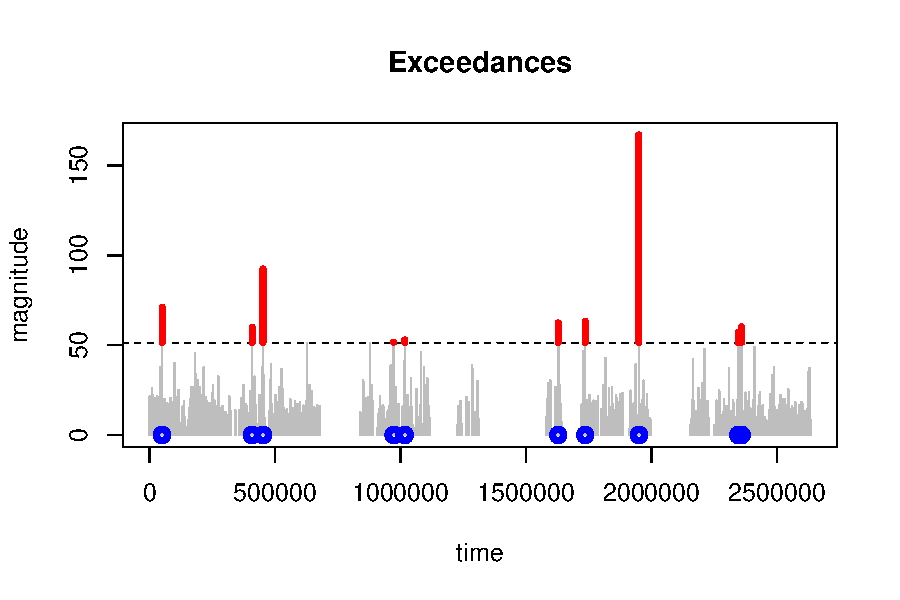
\includegraphics[scale=0.6]{Thesis/Figures/Exceedances.pdf}
        %\caption{Caption}
        %\label{fig:my_label}
    \end{figure}
    We are interested in modelling the durations $T_\ell := \inf\{t: M(N(t)) > \ell\}$ and the exceedances $X_\ell=M(N(T_\ell))-\ell$    
\end{frame}



\begin{frame}{Distribution of Exceedances and Exceedance Durations}
        Using the scaling limit theorem for our CTRM it can be shown that for large $\ell$
        \[
            T_\ell \sim ML(\beta,\delta),
        \]
	where ML refers to the Mittag-Leffler distribution. It can also be shown that
	\[
            X_\ell \sim GP(\xi,\tilde{\sigma}),
        \]
        where GP refers to the Generalised Pareto distribution.
\end{frame}

\section{Statistical Inference}

\begin{frame}{Threshold Selection}
At high thresholds we have a small amount of data points and thus a high variance.
\\~\\
Low thresholds introduce bias since exceedances and durations are only asymptotically GP and ML distributed.
\\~\\
We can transform all four parameters such that they're constant with respect to the threshold if the asymptotic approximations are accurate.
\\~\\
Thus we should pick the lowest threshold such that the transformed parameters remain constant.

\end{frame}

\begin{frame}{ A Possible Simulation }
	Waiting times $W_i$ are simulated according to a stable distribution with stability parameter $\alpha \in (0,1)$.
	\\~\\
	Jump sizes $J_i$ are simulated according to Generalized Extreme Value (GEV) distribution with location parameter $\mu$, scale parameter $\sigma$ and shape parameter $\xi$.
	\\~\\
	We can now test if our theoretical results hold for simulated data.
\end{frame}

\begin{frame}{Simulated data}
    \begin{center}
        $\alpha=0.4, \sigma=1, \xi=0.4$
    \end{center}
	\begin{figure}
        \centering
        \vspace{-0.5cm}
        \hspace{-0.8cm}
        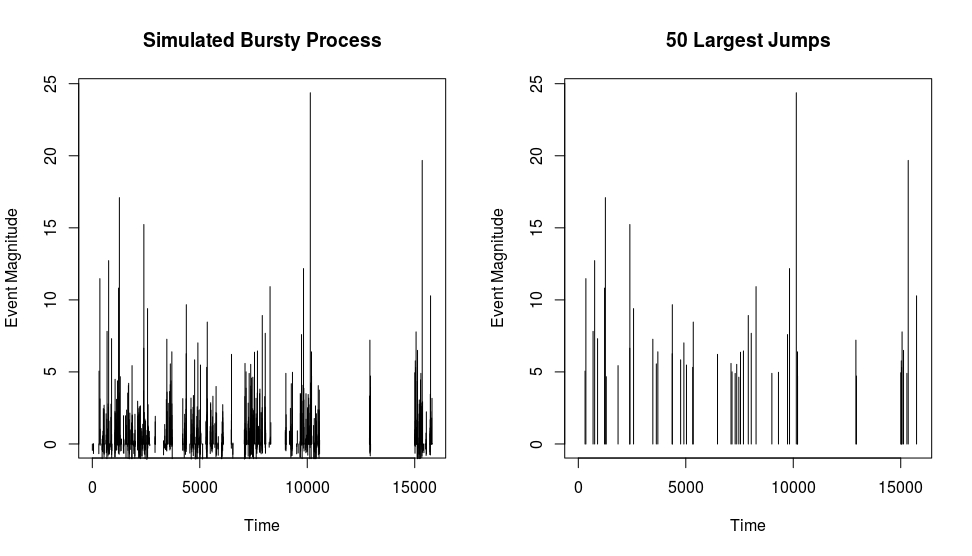
\includegraphics[scale=0.45]{SimulatedBursty.jpeg}
    \end{figure}
\end{frame}

\begin{frame}{Stability Plots}
    \begin{figure}
        \centering
        \vspace{-0.5cm}
        \hspace{-0cm}
        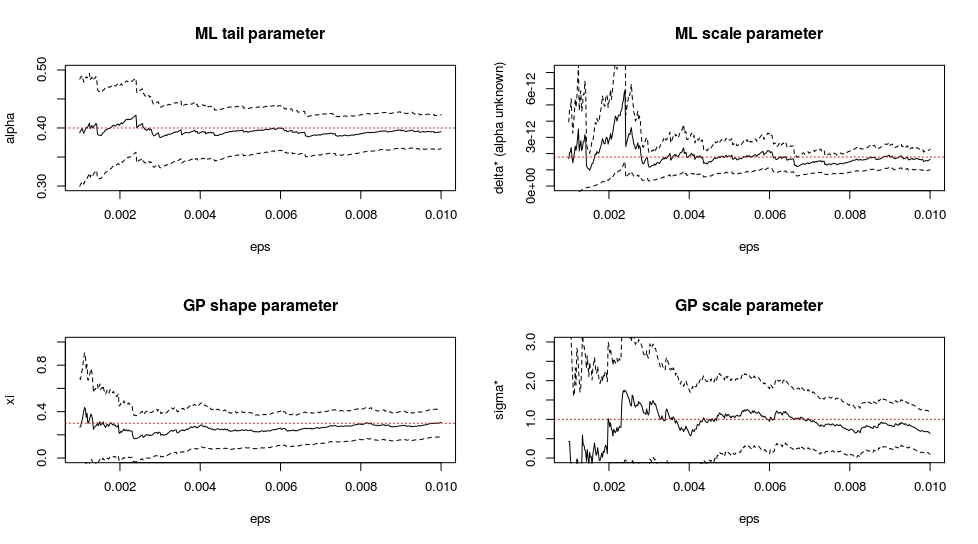
\includegraphics[scale=0.45]{Thesis/Figures/alphaUnknown}
    \end{figure}
\end{frame}


\begin{frame}{Further Research}
Apply the model to datasets with heavy tail waiting times such as bond futures trades, seismic activity and network transmissions.
\\~\\
Extend the model to include the case where there is a dependence structure between $W_i$ and $J_i$.
\end{frame}
 
\end{document}